\documentclass[titlepage,colorinlistoftodos]{article}
\usepackage{style}

\usepackage{float}
% \usepackage[hidelinks]{hyperref}
\usepackage{hyperref}
\usepackage{svg}
% \usepackage[disable]{todonotes}
\usepackage{todonotes}

\usepackage{listings}
\usepackage{xcolor}
\usepackage{pgfgantt}
\usepackage{pdflscape}

\begin{document}

\title{ADRIAN: Automated Decentralized Risk Assessment and Mitigation}
\author{Jorn J. Verhoeven}
\birthdate{January 10th, 1995}
\birthplace{Utrecht, The Netherlands}
\defensedate{September 11th, 2023 (Estimation)}
\supervisor{Dr. Z.A. Mann}
% \committeemember{Dr. C.U. Grelck}
\maketitle

\listoftodos{}
\newpage

\tableofcontents

\asJava % By default use Java as the code language

\section{Project Details}
\hspace{1.15em}
\textbf{Project title}: ADRIAN: Automated Decentralized Risk Assessment and Mitigation.

\textbf{Student name}: Jorn Verhoeven.

\textbf{Contact person}: Z.A. Mann (\href{mailto://z.a.mann@uva.nl}{z.a.mann@uva.nl}).

\textbf{Keywords}: Cybersecurity, Internet of Things (IoT), Risk Management, Risk Mitigation
\section{Project Summary}

The exponential growth of the internet has revolutionized several aspects of our modern life, such as communication, entertainment, and the way we work. However, this increasing level of connectivity also brings inherent security risks and breaches. These can compromise sensitive information and cause substantial financial and reputational damage to individuals and organizations. As a result, there is a growing need for effective and possibly automated risk management and network security measures to mitigate these risks.


In recent years, Common Vulnerabilities and Exposures (CVEs) have emerged as a critical component of risk management and network security. CVEs are publicly disclosed vulnerabilities and weaknesses that have been identified in software and hardware products. Each CVE is assigned a unique identification number, and detailed information about the vulnerability is published in a public database maintained by the National Cybersecurity and Communications Integration Center (NCCIC).
\add{Maybe add links to CVE and NCCIC}

By regularly monitoring the CVE database and applying software patches and updates to address known vulnerabilities, organizations can significantly reduce the risk of security breaches and other cyber threats. Failure to address known CVEs can leave systems vulnerable to a range of attacks, including malware infections, data breaches, and denial-of-service (DoS) attacks.

As of today, there are many vulnerability scanning tools available. Through this, any organizations can identify vulnerabilities in their applications and systems and prioritize them based on severity and potential impact. The software provides detailed information about each vulnerability, including its severity and potential impact. This information enables organizations to develop and implement effective mitigation strategies to address the identified vulnerabilities.

While these vulnerability scanners can be powerful tools for identifying and sometimes mitigating vulnerabilities in software applications and systems, they are limited in their ability to identify and address vulnerabilities that may exist beyond a single node of a network.

This is where \textbf{A}utomated \textbf{D}ecentralized \textbf{R}isk \textbf{A}ssessment and Mitigatio\textbf{N} (ADRIAN) could come into play. 
\section{Problem Analysis}
\section{Research Method}
The thesis will primarily focus on defining a \todo{Maybe get rid of 'functional'}functional protocol between agents to overcome the problems that were mentioned in the sections before. We think that by first creating an attack graph using predefined risk rules should allow any nodes within the network to assess the risk, in a localized portion of the network. We also think that allowing neighbouring agents to propose mitigations will reduce the overall risk of the network. 

To initiate, experiment with and refine the protocol we will perform a 
\begin{enumerate}
    \item Literature study
    \item Define hypotheses
    \item Experiments
\end{enumerate}

\subsection{Literature Study}
An initial literature study is done to investigate the current bleeding-edge technology and recent literature for risk assessment and mitigation strategies. The knowledge from this literature study will be applied to create a path that combines the hypothesized strengths (Subsection~\ref{ssec:hypothesis}) to a workable proof of concept. This proof of concept will then be used to evaluate the proposed protocol by running several experiments (Subsection~\ref{ssec:experiments}.

\subsection{Hypothesis} \label{ssec:hypothesis}
As explained in Section \ref{sec:problem-analysis}, existing research has been done to figure out ways of locally mitigating security risks. We however want to have a network of agents attempt to solve this problem together. We hypothesise that by letting agents within a network communicate and negotiate with one another according to our proposed protocol, that the overall risk probability of a network will decrease. 

We think that by having agents calculate Attack Graphs based on a local knowledge-base will allow the network to identify risks accurately and efficiently. We will experiment with different variables, such as the distance each agent can communicate (See Section \ref{ssec:experiments}), to analyze the impact of different strategies. This research aims to investigate the overall effect of this method, and will not be an exhaustive list of possible strategies. 

Additionally, we think that allowing agents to propose solutions to identified risks (through auctions) will decrease the overall risk probability. 


\subsection{Experiments} \label{ssec:experiments}
In order to validate the hypothesis, answer the research question a Proof of Concept (PoC) will be created as explained in Section \ref{sec:expected-results}. This PoC will allow us to execute several experiments in a controlled environment, where we can simulate different networks and events. Each experiment will be performed over multiple epochs. We define an epoch as a moment in time with an initial infrastructure which can be changed by agents by means of adaptations. This initial infrastructure can be different in each subsequent epoch, based on these mutations. No new infrastructure nodes or software components are added during an epoch. If mutations to the infrastructure should be considered, they are added to the initial infrastructure of the subsequent epoch.

\subsubsection{Control Experiment} 
To evaluate the quality of our proposed protocol we want to perform a control experiment. This experimental setup will allow nodes to apply predefined adaptation patterns to the properties and attributes of the node it is running on, just like in our proposal. However, the agents are not allowed to communicate with it's neighbours. What this will effectively simulate is a network in which agents will only identify and mitigate risks on it's own hosting node. 

In our controlled environment we can still calculate the overall risk probability and measure it over time. Thinks to consider when measuring are (but not limited to); Amount of adaptations, total number of risks identified, number of remaining risks.

\subsubsection{Broadcasting range}
Agents will be able to communicate with other agents in the network within an exchange range of \( Range(n) \), where \(n\) is a number representing the maximum distance (shortest path) between nodes. In our control experiment we effectively set \( Range(0) \) for the entire network, meaning that no knowledge is shared between nodes. \( Range(1) \) means that knowledge is shared between immediate neighbours. 
In this experiment we aim to evaluate the impact and cost of different knowledge exchange ranges. For this experiment we will attempt different ranges, and measure the effects over time. Thinks to consider when measuring are (but not limited to); Amount of adaptations, total number of messages exchanged, total number of risks identified, number of remaining risks.

\section{Expected Results} \label{sec:expected-results}
The results of this thesis are expected to be the following: 

\begin{enumerate}
    \item A Proof of Concept (PoC) which implements the conceptualized ADRIAN protocol, which used for simulation 
    \item Validation of ADRIAN through experimentation with the PoC.
    \item An assessment of possible strategies that can be used as an enhancement to the ADRIAN protocol.
\end{enumerate}
%\newpage
% \section{Required Expertise}
\section{Timeline} \label{sec:timeline}

\begin{landscape}

\begin{figure}[ht]

\begin{ganttchart}[
hgrid,
vgrid={*2dotted, red, *3dotted, red, *3dotted, red, *3dotted, red, *3dotted, red},
x unit=.6cm, 
y unit title=0.6cm,
y unit chart=0.6cm,
bar/.append style={fill=black!20},
bar label node/.append style=%
{align=left}
]{1}{19}
\gantttitle{Weeks}{19} \\
\gantttitlelist{18,...,36}{1} \\

\ganttgroup{Learning}{1}{6} \\
\ganttbar{Case-studies for relevant work}{1}{2} \\
\ganttbar{Graph Theory / Knowledge bases}{3}{5} \\

\ganttgroup{Code Implementation}{1}{14} \\
\ganttbar{Core Application Architecture}{1}{5} \\ 
\ganttbar{Knowledge Base}{4}{5} \\ 
\ganttbar{Attack Graph}{6}{7} \\ 
\ganttbar{Risk Assessment}{8}{9} \\
\ganttbar{Auctioning}{12}{13} \\ 

\ganttgroup{Experiment Execution}{4}{17} \\ 
\ganttbar{Initial Experiment Setup}{4}{7} \\ 
\ganttbar{RQ-1}{8}{11} \\ 
\ganttbar{RQ-2}{12}{15} \\ 
\ganttbar{Re-evaluation}{16}{17} \\

\ganttgroup{Thesis writing}{1}{19} \\
\ganttbar{Background \& Related work}{1}{6} \\
\ganttbar{Methodology}{4}{4}
\ganttbar{}{8}{8} 
\ganttbar{}{12}{12} \\
\ganttbar{Results \& evaluation}{7}{7}
\ganttbar{}{11}{11} 
\ganttbar{}{15}{15} \\
\ganttbar{Conclusion}{16}{18} \\
\ganttbar{Fine-tuning}{18}{19}

\end{ganttchart}

\caption{\label{fig::timeline}Thesis timeline}
\end{figure}
\end{landscape}


% Main content
%\section{Background}
\label{sec:background}
This section will briefly mention the background of this research, and will give a summary of the ADRIAN protocol. It will also detail the components of the ADRIAN protocol that are relevant to this research.

\subsection{ADRIAN Protocol}
\label{ssec:adrian}

As mentioned in the introduction, this research builds upon the earlier work of Mann and Smolka \cite{mann2023ADRIAN}. They propose a protocol, called \ADRIAN (or ADRIAN for short), which has the core objective to identify and mitigate risks in distributed systems, leveraging a decentralized and adaptive approach. Unlike conventional security frameworks that rely on a centralized authority to oversee system security, ADRIAN empowers autonomous software agents to collaboratively assess and address security risks. An abstract representation of the ADRIAN approach is shown in Figure \ref{fig:adrian-architecture}.

\begin{figure}
    \centering
    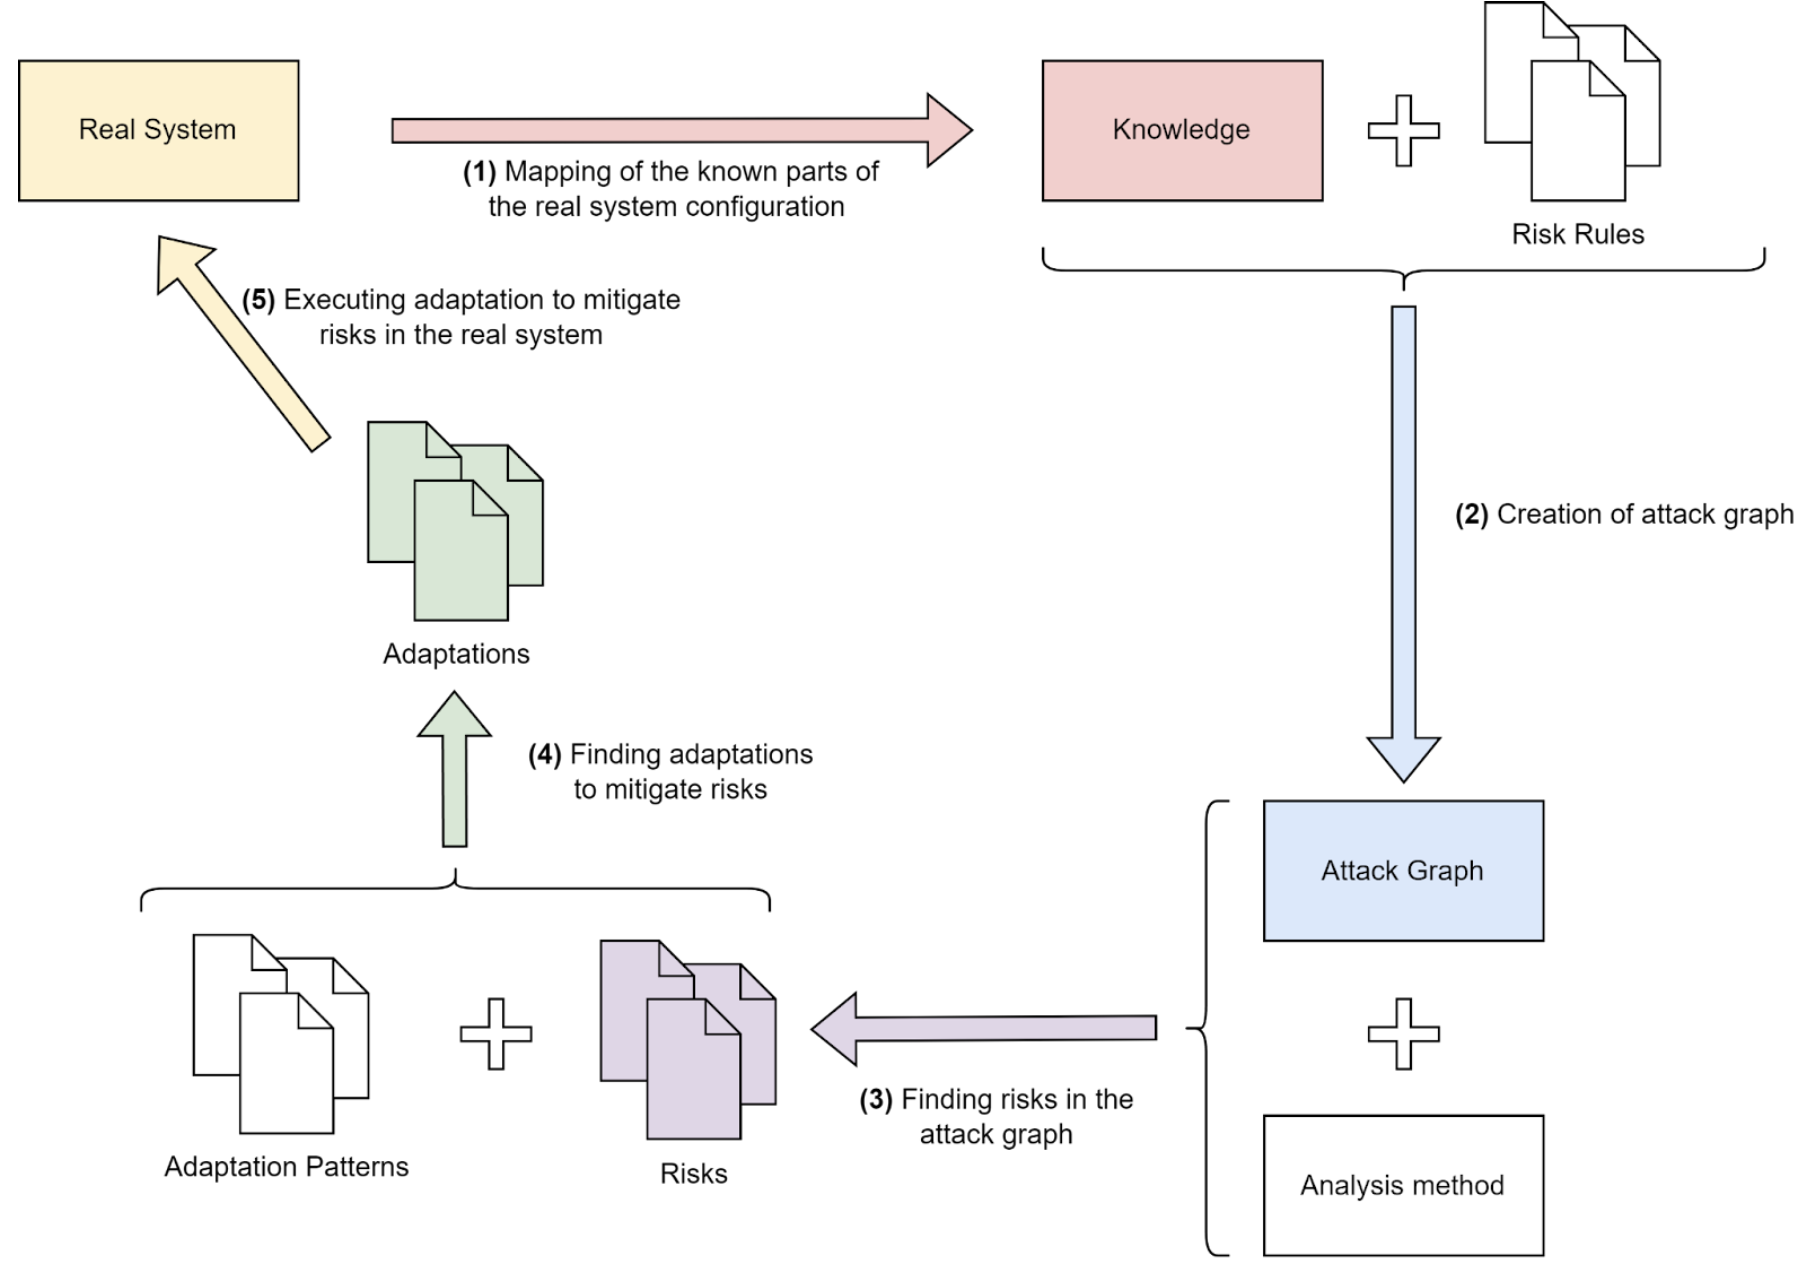
\includegraphics[width=0.8\textwidth]{content/adrian-architecture.png}
    \caption{The abstract representation of the ADRIAN approach. It shows how the different components interact with each other. This figure has been sourced from the ADRIAN concept by Mann and Smolka \cite{mann2023ADRIAN}.}
    \label{fig:adrian-architecture}
\end{figure}

In the ADRIAN protocol, agents are deployed across the infrastructure nodes of a network. These agents are responsible for monitoring the state of the node they are deployed on, specifically the properties of said node. These properties could range from firewall settings to OS and Firmware versions running on the node. Agents also know about the software that is deployed on their infrastructure node and its properties, such as SDK and software library versions, and if data is encrypted on disk. Some software components are marked as \emph{critical software}, indicating that the software contains important information or could lead to serious damage if compromised. All the information about the node and software is stored by the agent in a localized \emph{knowledge base}. Knowledge about each node, and it's software, is then exchanged between agents. This exchange will slowly propagate the knowledge throughout the network, allowing agents to have a more complete view of the network.

\vspace{0.5em}
To identify risks in a network an agent uses a set of \emph{risk rules}. These risk rules are based on known vulnerabilities, which are registered in the CVE list. They denote the probability of an attacker compromising the node/software. The definition of the risk rules that are implemented are detailed in Section \ref{ssec:risk-rules-adaptaions}.
These risk rules are then applied to the knowledge base to create \emph{attack graphs}, which are used to reason about the risk of a network. These attack graphs serve as a dynamic representation of the network's current status, where each node is represented as a vertex. Each edge ($n1 \rightarrow n2$) represents the risk that an attacker that can compromise $n1$, also manages to compromise $n2$. It is important to note that the attack graph is not an exact reflection of the real network; rather, it is a model derived from local observations and knowledge shared among agents. 
Note that sometimes vulnerabilities and risks are not yet registered as CVEs, but could exist in the real infrastructure. This means that the attack graph is not a 100\% accurate representation of the real world network, as it is not aware of these vulnerabilities. This is a problem, as it could lead to false negatives. However, this is a problem that is not unique to the ADRIAN protocol, as it is also present in other risk detection systems.

% \comment{Zoltan}{Critical software component is not explained yet.}
% \comment{Zoltan}{Risk report is not explained yet.}
% \comment{Zoltan}{Auction is not explainted yet.}
From the attack graph, agents can derive a set of \emph{critical paths}. These paths represent a path from an \emph{exposed node} to a critical software component. These critical paths are then used to determine the risk of a network and the potential damage that could be done which results in a \emph{risk report}. One of these risk reports is selected and will be \emph{auctioned} off to the agents in the network, more information about auctions is given below. In order to calculate the potential damage of a risk, the agent will combine all the probabilities of each individual edge of the attack graph along the critical path, using the following formula:

\[p = 1 - \prod_{k=1}^{R}(1-p_{k}) \]

Where $R$ is the number of all risks rules that lead to a risk edge between nodes a and b. $p_{k}$ is the probability of one of the risk rules from $R$. This formula gives us a single probability $p$ per edge. Calculating the product of all probabilities $p$ along the critical path, gets the final probability. This final probability is then multiplied with the critical software components damage (predetermined) to get the expected damage of the risk.

\vspace{0.5em}
The auctioning system is a mechanism that lets agents invite their peers to participate in the risk mitigation process. Once an agent has started an auction, other agents are invited to participate. These participating agents receive the risk report and attack graph as calculated by the initiating agent. Through a set of \emph{adaptation patterns}, agents can find multiple proposed solutions to reduce the potential damage of the risk report. These adaptation patterns are based on the risk rules, and describe possible adaptations that can be performed to mitigate the risk.
Each participating agent tries to find and select a proposal that mitigate the risk. This proposal is then sent back to the auctioneer agent, which will accumulate all proposals and select the proposal that is most beneficial to the network. The selected proposal is then executed by the agent that proposed it, and the network is updated accordingly.

%\input{thesis/sections/metrics}
%\input{thesis/sections/framework}
%
%
%\section{Discussion}
\label{sec:discussion}

\begin{figure}[H]
    \centering
    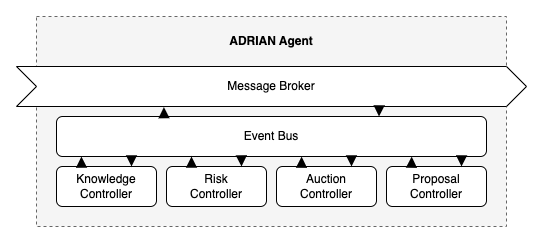
\includegraphics[width=0.8\textwidth]{_content/adrian-component-overview}
    \caption{Agent component overview}
    \label{fig:component-overview}
\end{figure}

\begin{figure}[H]
    \centering
    \includegraphics[width=0.8\textwidth]{_content/knowledge-sharing}
    \caption{Knowledge Exchange Sequence Diagram}
    \label{fig:knowledge-sharing}
\end{figure}


\begin{figure}[H]
    \centering
    \includegraphics[width=1.4\textwidth]{_content/auction}
    \caption{Auction Sequence Diagram}
    \label{fig:auction}
\end{figure}

%\section{Related Work}
\label{sec:related-work}

%\section{Conclusion}
\label{sec:conclusion}

At the start of this research we set out to answer the following research questions:

\vspace{0.5em}
\emph{Can the ADRIAN protocol be implemented and used for effective Risk Assessment and Mitigation?}
\vspace{0.5em}

Which would inturn be answered by the following questions: 
\begin{itemize}
    \item \textit{(Identification) Can we use the ADRIAN protocol to do automated risk identification within a network of nodes with an (imperfect) local knowledge base?}
    \item \textit{(Mitigation) Can the ADRIAN protocol be used to decrease the overall risk, by applying adaptation patterns over time?}
\end{itemize}

In this section we will answer these questions, with the information from the Result and Discussion sections in mind.

\paragraph*{Identification}
In Subsection \ref{ssec:risks-detected} we explained that the full implementation of the ADRIAN protocol is capable of detecting risks in a network of nodes. By using an internal knowledge base agents are able to detect risks that they would otherwise be unable to detect. The benefits of this decentralized approach are that agents only need to store, share, and assess the properties of each node for a subset of the problem. This makes it very scalable and allows for a large number of nodes to be added to the network. However, this also means that the agents are unable to detect risks that are outside of their knowledge base. This is a trade-off that is made in the ADRIAN protocol. 

\paragraph*{Mitigation}
The ADRIAN protocol, even without auctions, is able to decrease the overall risk and predicted damage of an infrastructure.
Subsections \ref{ssec:efficient-adaptations} and \ref{ssec:adaptation-time} explain that the full implementation of the ADRIAN protocol is capable of reducing the overall damage of the infrastructure, by using the concepts of auctions. These auctions allow agents to apply more effective adaptations, and reduce the amount of service-/downtime a node and its software components experience. 


\vspace{0.5em}
Combining all the information from Section \ref{sec:discussion} and the answers to the sub-research questions, we can conclude that the ADRIAN protocol can be used for effective risk assessment and mitigation. 

% Subsection \input{thesis/sections/f uture-work}
%

\bibliographystyle{abbrv}
\bibliography{bibliography}
\end{document}